\documentclass[border=20pt]{standalone}
\usepackage[T1]{fontenc}
\usepackage{tikz}
\usetikzlibrary{positioning, arrows.meta, shapes.geometric, fit, calc, backgrounds}
\usepackage{xcolor}

\definecolor{inputbg}{HTML}{E8F5E9}
\definecolor{stage1bg}{HTML}{E3F2FD}
\definecolor{stage2bg}{HTML}{FFF3E0}
\definecolor{stage3bg}{HTML}{E8F5E9}
\definecolor{outputbg}{HTML}{F3E5F5}
\definecolor{interpbg}{HTML}{FFF9C4}
\definecolor{toolcol}{HTML}{1565C0}
\definecolor{llmcol}{HTML}{C62828}
\definecolor{datacol}{HTML}{2E7D32}
\definecolor{arrowcol}{HTML}{455A64}
\definecolor{stageborder1}{HTML}{1976D2}
\definecolor{stageborder2}{HTML}{E65100}
\definecolor{stageborder3}{HTML}{2E7D32}
\definecolor{frontendcol}{HTML}{6A1B9A}
\definecolor{interpcol}{HTML}{F57F17}
\definecolor{gitcol}{HTML}{B71C1C}
\definecolor{riskcol}{HTML}{8E5EA2}
\definecolor{riskbg}{HTML}{F3E8FA}
\definecolor{qacol}{HTML}{1B5E20}

\tikzset{
  base/.style={rounded corners=5pt, draw, thick, align=center,
    font=\sffamily\footnotesize, minimum height=1.1cm, inner sep=8pt},
  input/.style={base, fill=inputbg, draw=datacol!80!black},
  tool/.style={base, fill=stage1bg, draw=toolcol, text=toolcol!90!black},
  subtool/.style={base, fill=stage1bg!50, draw=toolcol!60, text=toolcol!80!black, rounded corners=3pt},
  gittool/.style={base, fill=red!8, draw=gitcol!70, text=gitcol!90!black, rounded corners=3pt},
  risktool/.style={base, fill=riskbg, draw=riskcol!75!black, text=riskcol!95!black, rounded corners=3pt},
  data/.style={base, fill=white, draw=toolcol!75!black, text=toolcol!90!black, dashed},
  gitdata/.style={base, fill=red!5, draw=gitcol!60, text=gitcol!80!black, dashed},
  riskdata/.style={base, fill=riskbg!35, draw=riskcol!70!black, text=riskcol!90!black, dashed},
  interpbox/.style={base, fill=interpbg, draw=interpcol, text=interpcol!80!black, very thick, rounded corners=6pt},
  llm/.style={base, fill=stage2bg, draw=llmcol, text=llmcol!90!black, font=\sffamily\footnotesize\bfseries},
  qabox/.style={base, fill=stage3bg, draw=stageborder3, text=qacol!90!black, very thick, rounded corners=6pt},
  output/.style={base, fill=outputbg, draw=frontendcol, text=frontendcol!90!black},
  stagelab/.style={font=\sffamily\large\bfseries, text=#1},
  stagesub/.style={font=\sffamily\scriptsize\itshape, text=black!55},
  arr/.style={-{Stealth[length=6pt,width=5pt]}, thick, arrowcol},
  bigarr/.style={-{Stealth[length=8pt,width=7pt]}, very thick},
  dataarr/.style={-{Stealth[length=5pt,width=4pt]}, thick, toolcol!75!black},
  gitarr/.style={-{Stealth[length=5pt,width=4pt]}, thick, gitcol!75!black},
  riskarr/.style={-{Stealth[length=5pt,width=4pt]}, thick, riskcol!80!black},
  arrlabel/.style={font=\sffamily\scriptsize\bfseries, text=arrowcol, fill=white, inner sep=2pt, rounded corners=1pt},
}

%=======================================================================
% LAYOUT PLAN (all cm)
%
% All boxes use minimum width=3.6cm (half=1.8) or 4.6cm (half=2.3), etc.
% I'll track LEFT and RIGHT edges explicitly.
%
%  LLM Frontend  cx=0,   hw=2.3  → x=[-2.3, +2.3]
%  Git Repo      cx=7,   hw=1.9  → x=[5.1, 8.9]
%  Orch          cx=14,  hw=2.5  → x=[11.5, 16.5]  y=0
%
%  -- Tool row (y=-6.5) --
%  NeoDepends    cx=11,  hw=1.9  → x=[9.1, 12.9]
%  DV8 Console   cx=17,  hw=2.1  → x=[14.9, 19.1]
%
%  -- Git tool row (y=-12) --  MOVED LEFT to cx=3, away from data col
%  fetch_issues  cx=3,   hw=2.1  → x=[0.9, 5.1]
%
%  -- DV8 data col cx=23, hw=1.8 → x=[21.2, 24.8]
%  -- issue_map same col, y=-9.5
%
%  -- Process col cx=30, hw=2.3  → x=[27.7, 32.3]
%  -- Output JSON cx=37, hw=1.8  → x=[35.2, 38.8]
%
% ARROW LANES:
%  L1 = x=6.5   (right of fetch_issues.east=5.1, left of depends.west=9.1)
%                Used for: repo.south → fetch_issues drop, then fetch_issues.east → issue_map
%  L2 = x=10.0  (left of orch.west=11.5, right of depends=9.1..12.9)
%                Used for: orch → depends drop
%  L3 = x=18.0  (right of orch.east=16.5, left of dv8.east=19.1) — too tight
%                Actually: orch → dv8: orch.south → down to y=-3.5 → right to cx=17 → dv8.north
%  L4 = x=20.5  (right of dv8.east=19.1, left of data.west=21.2)
%                Used for: DV8 → data boxes fan-out trunk
%  L5 = x=25.5  (right of data.east=24.8, left of process.west=27.7)
%                Used for: data boxes → payload, data boxes → evidiff
%                apdata/hotdata → riskscores use sub-lane x=25.0
%  L6 = x=33.5  (right of process.east=32.3, left of output.west=35.2)
%                write arrows
%  L7 = x=40.5  (right of output.east=38.8, left of interpdata.west~42.3)
%                output JSONs → interpdata
%=======================================================================

\begin{document}
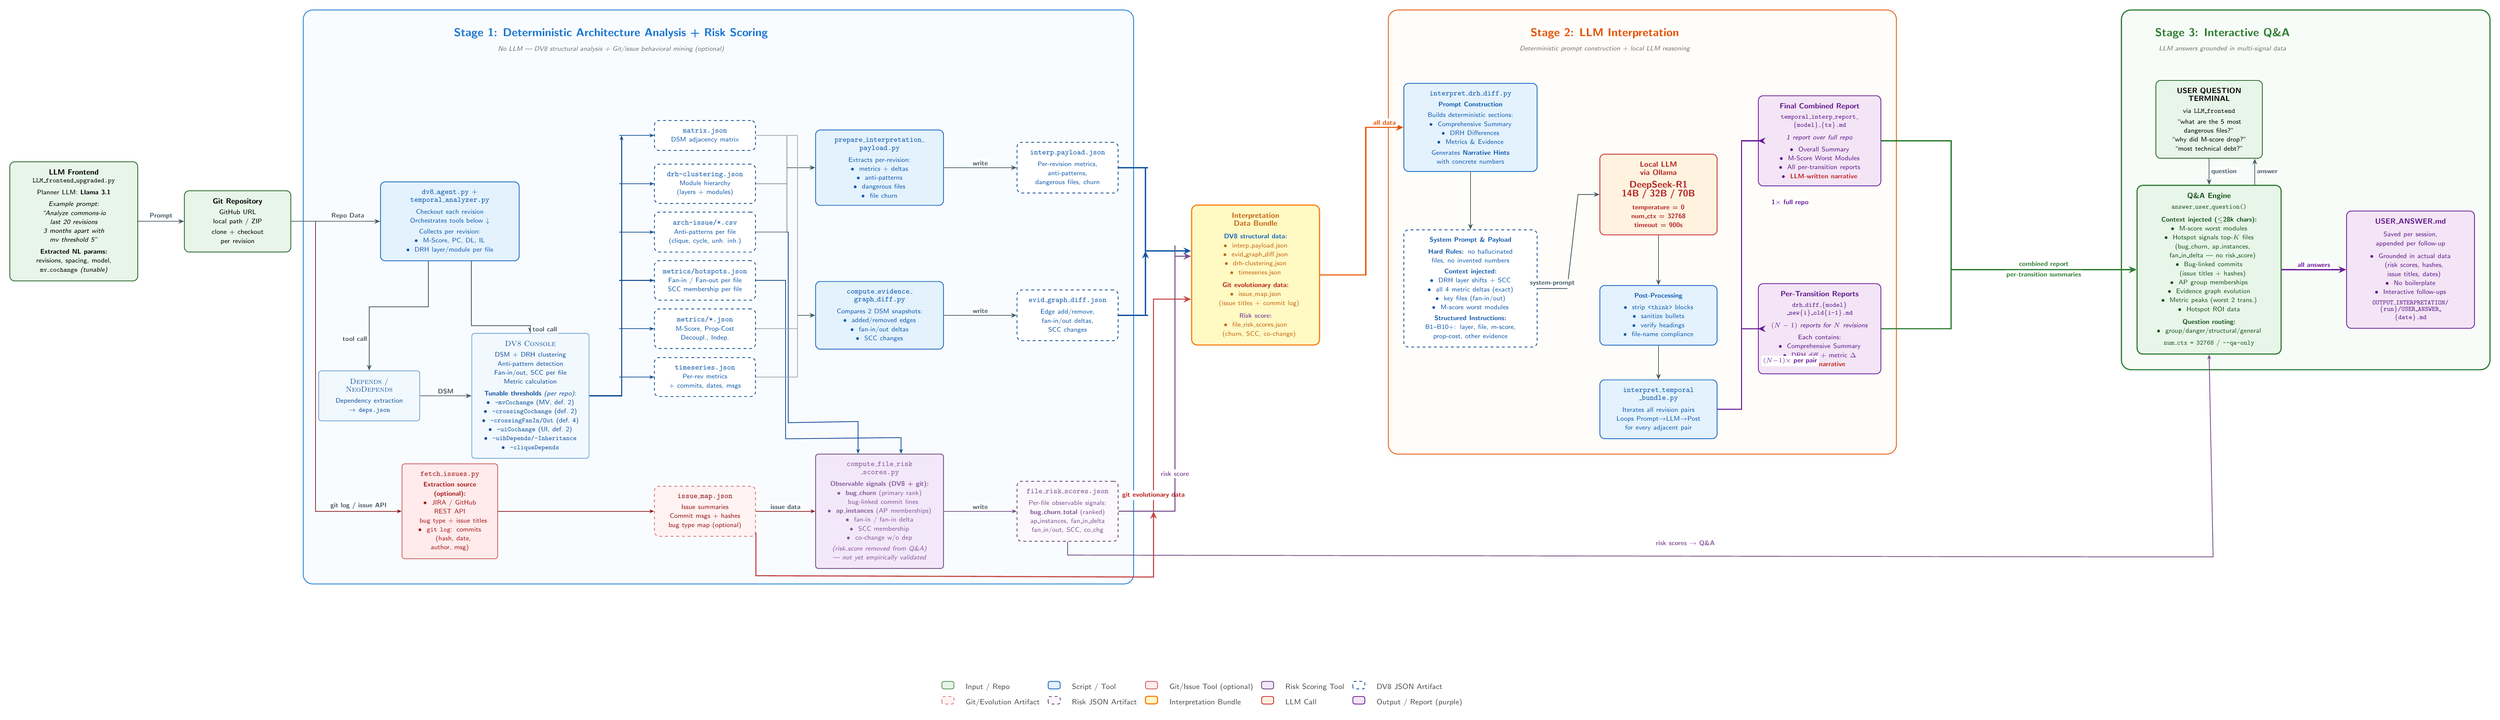
\begin{tikzpicture}

%----------------------------------------------------------------------
% INPUT NODES
%----------------------------------------------------------------------
\node[input, text width=4.2cm, minimum width=4.6cm] at (0,0) (frontend)
  {\textbf{LLM Frontend}\\[-1pt]{\scriptsize\texttt{LLM\_frontend\_upgraded.py}}\\[3pt]
   {\scriptsize Planner LLM: \textbf{Llama 3.1}}\\[3pt]
   {\scriptsize\itshape Example prompt:}\\
   {\scriptsize\itshape ``Analyze commons-io}\\
   {\scriptsize\itshape last 20 revisions}\\
   {\scriptsize\itshape 3 months apart with}\\
   {\scriptsize\itshape mv threshold 5''}\\[3pt]
   {\scriptsize \textbf{Extracted NL params:}}\\
   {\scriptsize revisions, spacing, model,}\\
   {\scriptsize \texttt{mv\_cochange} \textit{(tunable)}}};
% frontend: hw=2.3 → x=[-2.3,+2.3]

\node[input, text width=3.4cm, minimum width=3.8cm] at (6.1,0) (repo)
  {\textbf{Git Repository}\\[2pt]
   {\scriptsize GitHub URL}\\
   {\scriptsize local path / ZIP}\\[2pt]
   {\scriptsize clone + checkout}\\
   {\scriptsize per revision}};
% repo: hw=1.9 → x=[5.1,8.9]

%----------------------------------------------------------------------
% STAGE 1 — ORCHESTRATOR  cx=14
%----------------------------------------------------------------------
\node[tool, text width=4.6cm, minimum width=5.0cm] at (14,0) (orch)
  {\texttt{dv8\_agent.py} +\\[-1pt]\texttt{temporal\_analyzer.py}\\[3pt]
   {\scriptsize Checkout each revision}\\
   {\scriptsize Orchestrates tools below $\downarrow$}\\[2pt]
   {\scriptsize Collects per revision:}\\
   {\scriptsize \textbullet\; M-Score, PC, DL, IL}\\
   {\scriptsize \textbullet\; DRH layer/module per file}};
% orch: hw=2.5 → x=[11.5,16.5]  top~+1.6 bot~-1.6

% NeoDepends  cx=11, y=-6.5
\node[subtool, text width=3.2cm, minimum width=3.6cm] at (11,-6.5) (depends)
  {\textsc{Depends /}\\[-1pt]\textsc{NeoDepends}\\[2pt]
   {\scriptsize Dependency extraction}\\
   {\scriptsize $\to$ \texttt{deps.json}}};
% depends: hw=1.8 → x=[9.2,12.8]  top=-5.7 bot=-7.3

% DV8 Console  cx=17, y=-6.5
\node[subtool, text width=3.8cm, minimum width=4.2cm] at (17,-6.5) (dv8)
  {\textsc{DV8 Console}\\[2pt]
   {\scriptsize DSM + DRH clustering}\\
   {\scriptsize Anti-pattern detection}\\
   {\scriptsize Fan-in/out, SCC per file}\\
   {\scriptsize Metric calculation}\\[3pt]
   {\scriptsize \textbf{Tunable thresholds} \textit{(per repo)}:}\\
   {\scriptsize \textbullet\; \texttt{-mvCochange} (MV, def.\ 2)}\\
   {\scriptsize \textbullet\; \texttt{-crossingCochange} (def.\ 2)}\\
   {\scriptsize \textbullet\; \texttt{-crossingFanIn/Out} (def.\ 4)}\\
   {\scriptsize \textbullet\; \texttt{-uiCochange} (UI, def.\ 2)}\\
   {\scriptsize \textbullet\; \texttt{-uihDepends/-Inheritance}}\\
   {\scriptsize \textbullet\; \texttt{-cliqueDepends}}};
% dv8: hw=2.1 → x=[14.9,19.1]  top=-5.6 bot=-7.4

% fetch_issues centered under dv8_agent.py
\node[gittool, text width=3.0cm, minimum width=3.4cm] at (14,-10.8) (fetchissues)
  {\texttt{fetch\_issues.py}\\[2pt]
   {\scriptsize \textbf{Extraction source (optional):}}\\
   {\scriptsize \textbullet\; JIRA / GitHub REST API}\\
   {\scriptsize \quad bug type + issue titles}\\
   {\scriptsize \textbullet\; \texttt{git log}: commits}\\
   {\scriptsize \quad (hash, date, author, msg)}};
% fetchissues: centered on x=14

%----------------------------------------------------------------------
% DV8 DATA COLUMN  cx=23
% 6 boxes: y = 3.2, 1.4, -0.4, -2.2, -4.0, -5.8
% issue_map: y=-8.0
% box hw=1.8 → x=[21.2,24.8]
%----------------------------------------------------------------------
\node[data, text width=3.2cm, minimum width=3.6cm] at (23.5, 3.2)  (dsm)
  {\texttt{matrix.json}\\{\scriptsize DSM adjacency matrix}};
\node[data, text width=3.2cm, minimum width=3.6cm] at (23.5, 1.4)  (drh)
  {\texttt{drh-clustering.json}\\{\scriptsize Module hierarchy}\\{\scriptsize (layers + modules)}};
\node[data, text width=3.2cm, minimum width=3.6cm] at (23.5,-0.4)  (apdata)
  {\texttt{arch-issue/*.csv}\\{\scriptsize Anti-patterns per file}\\{\scriptsize (clique, cycle, unh.~inh.)}};
\node[data, text width=3.2cm, minimum width=3.6cm] at (23.5,-2.2)  (hotdata)
  {\texttt{metrics/hotspots.json}\\{\scriptsize Fan-in / Fan-out per file}\\{\scriptsize SCC membership per file}};
\node[data, text width=3.2cm, minimum width=3.6cm] at (23.5,-4.0)  (metrics)
  {\texttt{metrics/*.json}\\{\scriptsize M-Score, Prop-Cost}\\{\scriptsize Decoupl., Indep.}};
\node[data, text width=3.2cm, minimum width=3.6cm] at (23.5,-5.8)  (timeseries)
  {\texttt{timeseries.json}\\{\scriptsize Per-rev metrics}\\{\scriptsize + commits, dates, msgs}};
\node[gitdata, text width=3.2cm, minimum width=3.6cm] at (23.5,-10.8) (issuemap)
  {\texttt{issue\_map.json}\\[2pt]
   {\scriptsize Issue summaries}\\
   {\scriptsize Commit msgs + hashes}\\
   {\scriptsize bug type map (optional)}};
% issuemap: top=-7.1 bot=-8.9

%----------------------------------------------------------------------
% PROCESS SCRIPTS COLUMN  cx=30
% payload y=2.0, evidiff y=-3.5, riskscores y=-8.0
% hw=2.3 → x=[27.7,32.3]
%----------------------------------------------------------------------
\node[tool, text width=4.2cm, minimum width=4.6cm] at (30, 2.0) (payload)
  {\texttt{prepare\_interpretation\_}\\[-1pt]\texttt{payload.py}\\[3pt]
   {\scriptsize Extracts per-revision:}\\
   {\scriptsize \textbullet\; metrics + deltas}\\
   {\scriptsize \textbullet\; anti-patterns}\\
   {\scriptsize \textbullet\; dangerous files}\\
   {\scriptsize \textbullet\; file churn}};
% payload: top~+3.8 bot~+0.2

\node[tool, text width=4.2cm, minimum width=4.6cm] at (30,-3.5) (evidiff)
  {\texttt{compute\_evidence\_}\\[-1pt]\texttt{graph\_diff.py}\\[3pt]
   {\scriptsize Compares 2 DSM snapshots:}\\
   {\scriptsize \textbullet\; added/removed edges}\\
   {\scriptsize \textbullet\; fan-in/out deltas}\\
   {\scriptsize \textbullet\; SCC changes}};
% evidiff: top~-2.0 bot~-5.0

\node[risktool, text width=4.2cm, minimum width=4.6cm] at (30,-10.8) (riskscores)
  {\texttt{compute\_file\_risk}\\[-1pt]\texttt{\_scores.py}\\[3pt]
   {\scriptsize \textbf{Observable signals (DV8 + git):}}\\
   {\scriptsize \textbullet\; \textbf{bug\_churn} (primary rank)}\\
   {\scriptsize \quad bug-linked commit lines}\\
   {\scriptsize \textbullet\; \textbf{ap\_instances} (AP memberships)}\\
   {\scriptsize \textbullet\; fan-in / fan-in delta}\\
   {\scriptsize \textbullet\; SCC membership}\\
   {\scriptsize \textbullet\; co-change w/o dep}\\[2pt]
   {\scriptsize \textit{(risk\_score removed from Q\&A)}}\\
   {\scriptsize \textit{--- not yet empirically validated}}};
% riskscores: top~-6.3 bot~-9.7

%----------------------------------------------------------------------
% OUTPUT JSON COLUMN  cx=37
% same y-levels as their scripts
% hw=1.8 → x=[35.2,38.8]
%----------------------------------------------------------------------
\node[data, text width=3.2cm, minimum width=3.6cm] at (37, 2.0) (interpjson)
  {\texttt{interp\_payload.json}\\[3pt]
   {\scriptsize Per-revision metrics,}\\
   {\scriptsize anti-patterns,}\\
   {\scriptsize dangerous files, churn}};

\node[data, text width=3.2cm, minimum width=3.6cm] at (37,-3.5) (evidjson)
  {\texttt{evid\_graph\_diff.json}\\[3pt]
   {\scriptsize Edge add/remove,}\\
   {\scriptsize fan-in/out deltas,}\\
   {\scriptsize SCC changes}};

\node[riskdata, text width=3.2cm, minimum width=3.6cm] at (37,-10.8) (riskjson)
  {\texttt{file\_risk\_scores.json}\\[3pt]
   {\scriptsize Per-file observable signals:}\\
   {\scriptsize \textbf{bug\_churn\_total} (ranked)}\\
   {\scriptsize ap\_instances, fan\_in\_delta}\\
   {\scriptsize fan\_in/out, SCC, co\_chg}};

% Stage 1 title
\node[stagelab=stageborder1] at (20, 7.0) (s1title)
  {Stage 1: Deterministic Architecture Analysis + Risk Scoring};
\node[stagesub, below=1pt of s1title] (s1sub)
  {No LLM --- DV8 structural analysis + Git/issue behavioral mining (optional)};

\begin{scope}[on background layer]
  \node[fill=stage1bg!20, rounded corners=10pt, draw=stageborder1, thick,
    fit=(s1title)(s1sub)(orch)(depends)(dv8)(fetchissues)
        (dsm)(drh)(apdata)(hotdata)(metrics)(timeseries)(issuemap)
        (payload)(evidiff)(riskscores)(interpjson)(evidjson)(riskjson),
    inner sep=16pt] (s1box) {};
\end{scope}

%----------------------------------------------------------------------
% INTERPRETATION DATA BUNDLE  cx=44
%----------------------------------------------------------------------
\node[interpbox, text width=4.2cm, minimum width=4.6cm] at (44,-2.0) (interpdata)
  {\textbf{Interpretation}\\[-1pt]\textbf{Data Bundle}\\[4pt]
   {\scriptsize \textcolor{toolcol}{\textbf{DV8 structural data:}}}\\
   {\scriptsize \textbullet\; interp\_payload.json}\\
   {\scriptsize \textbullet\; evid\_graph\_diff.json}\\
   {\scriptsize \textbullet\; drh-clustering.json}\\
   {\scriptsize \textbullet\; timeseries.json}\\[4pt]
   {\scriptsize \textcolor{gitcol}{\textbf{Git evolutionary data:}}}\\
   {\scriptsize \textbullet\; issue\_map.json}\\
   {\scriptsize \quad (issue titles + commit log)}\\[4pt]
   {\scriptsize \textcolor{riskcol}{\textbf{Risk score:}}}\\
   {\scriptsize \textbullet\; file\_risk\_scores.json}\\
   {\scriptsize \quad (churn, SCC, co-change)}};
% interpdata: hw=2.3 → x=[41.7,46.3]

%----------------------------------------------------------------------
% STAGE 2
%----------------------------------------------------------------------
\node[tool, text width=4.4cm, minimum width=4.8cm] at (52, 3.5) (promptbuild)
  {\texttt{interpret\_drh\_diff.py}\\[2pt]
   {\scriptsize \textbf{Prompt Construction}}\\[2pt]
   {\scriptsize Builds deterministic sections:}\\
   {\scriptsize \textbullet\; Comprehensive Summary}\\
   {\scriptsize \textbullet\; DRH Differences}\\
   {\scriptsize \textbullet\; Metrics \& Evidence}\\[2pt]
   {\scriptsize Generates \textbf{Narrative Hints}}\\
   {\scriptsize with concrete numbers}};
% promptbuild: hw=2.4 → x=[49.6,54.4]

\node[data, text width=4.4cm, minimum width=4.8cm] at (52,-2.5) (promptdata)
  {\textbf{\scriptsize System Prompt \& Payload}\\[3pt]
   {\scriptsize \textbf{Hard Rules:} no hallucinated}\\
   {\scriptsize files, no invented numbers}\\[2pt]
   {\scriptsize \textbf{Context injected:}}\\
   {\scriptsize \textbullet\; DRH layer shifts + SCC}\\
   {\scriptsize \textbullet\; all 4 metric deltas (exact)}\\
   {\scriptsize \textbullet\; key files (fan-in/out)}\\
   {\scriptsize \textbullet\; M-score worst modules}\\[2pt]
   {\scriptsize \textbf{Structured Instructions:}}\\
   {\scriptsize B1--B10+: layer, file, m-score,}\\
   {\scriptsize prop-cost, other evidence}};
% promptdata: hw=2.4 → x=[49.6,54.4]

\node[llm, text width=3.8cm, minimum width=4.2cm] at (59, 1.0) (llmcall)
  {\textbf{Local LLM}\\[-1pt]\textbf{via Ollama}\\[4pt]
   {\normalsize DeepSeek-R1}\\
   {\normalsize 14B / 32B / \textbf{70B}}\\[4pt]
   {\scriptsize temperature = 0}\\
   {\scriptsize num\_ctx = 32768}\\
   {\scriptsize timeout = 900s}};
% llmcall: hw=2.1 → x=[56.9,61.1]

\node[tool, text width=3.8cm, minimum width=4.2cm] at (59,-3.5) (postproc)
  {\textbf{\scriptsize Post-Processing}\\[3pt]
   {\scriptsize \textbullet\; strip \texttt{<think>} blocks}\\
   {\scriptsize \textbullet\; sanitize bullets}\\
   {\scriptsize \textbullet\; verify headings}\\
   {\scriptsize \textbullet\; file-name compliance}};

\node[tool, text width=3.8cm, minimum width=4.2cm] at (59,-7.0) (bundle)
  {\texttt{interpret\_temporal}\\[-1pt]\texttt{\_bundle.py}\\[3pt]
   {\scriptsize Iterates all revision pairs}\\
   {\scriptsize Loops Prompt$\to$LLM$\to$Post}\\
   {\scriptsize for every adjacent pair}};
% bundle: hw=2.1 → x=[56.9,61.1]  bot~-8.5

\node[output, text width=4.0cm, minimum width=4.4cm] at (65, 3.0) (finalout)
  {\textbf{Final Combined Report}\\[3pt]
   {\scriptsize\texttt{temporal\_interp\_report\_}\\[-1pt]\texttt{\{model\}\_\{ts\}.md}}\\[4pt]
   {\scriptsize \textit{1 report over full repo}}\\[3pt]
   {\scriptsize \textbullet\; Overall Summary}\\
   {\scriptsize \textbullet\; M-Score Worst Modules}\\
   {\scriptsize \textbullet\; All per-transition reports}\\
   {\scriptsize \textbullet\; \textcolor{llmcol}{\textbf{LLM-written narrative}}}};
% finalout: hw=2.2 → x=[62.8,67.2]

\node[output, text width=4.0cm, minimum width=4.4cm] at (65,-4.0) (pertrans)
  {\textbf{Per-Transition Reports}\\[3pt]
   {\scriptsize \texttt{drh\_diff\_\{model\}}\\[-1pt]\texttt{\_new\{i\}\_old\{i-1\}.md}}\\[4pt]
   {\scriptsize \textit{$(N-1)$ reports for $N$ revisions}}\\[3pt]
   {\scriptsize Each contains:}\\
   {\scriptsize \textbullet\; Comprehensive Summary}\\
   {\scriptsize \textbullet\; DRH diff + metric $\Delta$}\\
   {\scriptsize \textbullet\; \textcolor{llmcol}{\textbf{LLM narrative}}}};

\node[stagelab=stageborder2] at (57, 7.0) (s2title)
  {Stage 2: LLM Interpretation};
\node[stagesub, below=1pt of s2title] (s2sub)
  {Deterministic prompt construction + local LLM reasoning};

\begin{scope}[on background layer]
  \node[fill=stage2bg!20, rounded corners=10pt, draw=stageborder2, thick,
    fit=(s2title)(s2sub)(promptbuild)(promptdata)(llmcall)(postproc)(bundle)(finalout)(pertrans),
    inner sep=16pt] (s2box) {};
\end{scope}

%----------------------------------------------------------------------
% STAGE 3
%----------------------------------------------------------------------
\node[input, text width=3.4cm, minimum width=3.8cm] at (79.5,3.8) (userq)
  {\textbf{USER QUESTION}\\[-1pt]\textbf{TERMINAL}\\[3pt]
   {\scriptsize via \texttt{LLM\_frontend}}\\[2pt]
   {\scriptsize ``what are the 5 most}\\
   {\scriptsize dangerous files?''}\\
   {\scriptsize ``why did M-score drop?''}\\
   {\scriptsize ``most technical debt?''}};

\node[qabox, text width=4.8cm, minimum width=5.2cm] at (79.5,-1.8) (qaengine)
  {\textbf{Q\&A Engine}\\[2pt]
   {\scriptsize \texttt{answer\_user\_question()}}\\[4pt]
   {\scriptsize \textbf{Context injected ($\leq$28k chars):}}\\
   {\scriptsize \textbullet\; M-score worst modules}\\
   {\scriptsize \textbullet\; Hotspot signals top-$K$ files}\\
   {\scriptsize \quad (bug\_churn, ap\_instances,}\\
   {\scriptsize \quad fan\_in\_delta --- no risk\_score)}\\
   {\scriptsize \textbullet\; Bug-linked commits}\\
   {\scriptsize \quad (issue titles + hashes)}\\
   {\scriptsize \textbullet\; AP group memberships}\\
   {\scriptsize \textbullet\; Evidence graph evolution}\\
   {\scriptsize \textbullet\; Metric peaks (worst 2 trans.)}\\
   {\scriptsize \textbullet\; Hotspot ROI data}\\[4pt]
   {\scriptsize \textbf{Question routing:}}\\
   {\scriptsize \textbullet\; group/danger/structural/general}\\[3pt]
   {\scriptsize \texttt{num\_ctx = 32768} / \texttt{--qa-only}}};
% qaengine: hw=2.5 → x=[77.0,82.0]

\node[output, text width=4.2cm, minimum width=4.6cm] at (87,-1.8) (qaout)
  {\textbf{USER\_ANSWER.md}\\[4pt]
   {\scriptsize Saved per session,}\\
   {\scriptsize appended per follow-up}\\[4pt]
   {\scriptsize \textbullet\; Grounded in actual data}\\
   {\scriptsize \quad (risk scores, hashes,}\\
   {\scriptsize \quad issue titles, dates)}\\
   {\scriptsize \textbullet\; No boilerplate}\\
   {\scriptsize \textbullet\; Interactive follow-ups}\\[3pt]
   {\scriptsize \texttt{OUTPUT\_INTERPRETATION/}\\[-1pt]
   \texttt{\{run\}/USER\_ANSWER\_}\\[-1pt]
   \texttt{\{date\}.md}}};

\node[stagelab=stageborder3] at (80, 7.0) (s3title)
  {Stage 3: Interactive Q\&A};
\node[stagesub, below=1pt of s3title] (s3sub)
  {LLM answers grounded in multi-signal data};

\begin{scope}[on background layer]
  \node[fill=stage3bg!30, rounded corners=10pt, draw=stageborder3, very thick,
    fit=(s3title)(s3sub)(userq)(qaengine)(qaout),
    inner sep=16pt] (s3box) {};
\end{scope}

%======================================================================
% ARROWS — ALL STRICTLY ORTHOGONAL
%
% Box edges (half-widths from centre x):
%  frontend  cx=0,   hw=2.3  → right=2.3
%  repo      cx=7,   hw=1.9  → left=5.1, right=8.9, bot≈-1.1, top≈+1.1
%  orch      cx=14,  hw=2.5  → left=11.5, right=16.5, top≈+1.8, bot≈-1.8
%  depends   cx=11,  hw=1.8  → left=9.2, right=12.8, top≈-5.7, bot≈-7.3
%  dv8       cx=17,  hw=2.1  → left=14.9, right=19.1, top≈-5.6, bot≈-7.4
%  fetchiss  cx=3,   hw=2.1  → left=0.9, right=5.1, top≈-8.9, bot≈-11.1
%  data col  cx=23,  hw=1.8  → left=21.2, right=24.8
%  process   cx=30,  hw=2.3  → left=27.7, right=32.3
%  output    cx=37,  hw=1.8  → left=35.2, right=38.8
%  interpdata cx=44, hw=2.3  → left=41.7, right=46.3
%
% DEDICATED ARROW LANES (vertical trunks, x-values):
%  Lane A  x=19.5  DV8.east trunk (between dv8.right=19.1 and data.left=21.2)
%  Lane B  x=25.8  data→payload/evidiff  (between data.right=24.8 and process.left=27.7)
%  Lane C  x=26.5  apdata/hotdata→riskscores  (same gap, slightly right of B)
%  Lane D  x=40.2  JSONs→interpdata  (between output.right=38.8 and interpdata.left=41.7)
%  Lane E  x=48.0  interpdata→Stage2  (between interpdata.right=46.3 and prompt.left=49.6)
%  Lane F  x=57.2  promptdata→llmcall  (between prompt.right=54.4 and llmcall.left=56.9)
%  Lane G  x=62.8  bundle→reports  (right of bundle.right=61.1)
%  Lane H  x=69.8  reports→QAengine
%
% HORIZONTAL LANES (y-values for long horizontal runs):
%  H1  y=+5.5  above all boxes (DV8 trunk up to dsm)
%  H2  y=-4.0  orch→depends/dv8 split (below orch.bot=-1.8, above depends.top=-5.7)
%  H3  y=-12.0 below all boxes (fetch_issues→issuemap, issuemap→interpdata, riskjson→QA)
%======================================================================

% Frontend → Repo
\draw[arr] (frontend.east) -- node[arrlabel,above]{Prompt} (repo.west);
% Repo → Orchestrator
\coordinate (repobranch) at (9.0,0);
\draw[arr] (repo.east) -- (repobranch) -- node[arrlabel,above]{Repo Data} (orch.west);

%-- Repo → fetch_issues ---------------------------------------------------
% Split from the repo-data lane before the Depends box, then route down and right.
\draw[gitarr] (repobranch)
  -- ++(0,-10.8)
  -- node[arrlabel,above]{\scriptsize git log / issue API}
     (fetchissues.west);

%-- Orch → NeoDepends -----------------------------------------------------
% Exit from orch.south offset LEFT (-0.8) to separate from DV8 arrow
% Route: (13.2,-1.8) → down to (13.2,-3.5) → left to (11,-3.5) → down to depends.north(11,-5.7)
% y=-3.5: below orch.bot=-1.8 ✓, above depends.top=-5.7 ✓
\draw[arr] ([xshift=-8mm]orch.south)
  -- ++(0,-1.7)              % (13.2,-3.5)
  -- ++(-2.2,0)               % (11.0,-3.5)
  -- node[arrlabel,left]{\scriptsize tool call} (depends.north);

%-- Orch → DV8 Console ----------------------------------------------------
% Exit from orch.south offset RIGHT (+0.8) to separate from NeoDepends arrow
% Route: (14.8,-1.8) → down to (14.8,-4.2) → right to (17,-4.2) → down to dv8.north(17,-5.6)
% y=-4.2: below orch.bot=-1.8 ✓, above dv8.top=-5.6 ✓, different y from NeoDepends lane ✓
\draw[arr] ([xshift=+8mm]orch.south)
  -- ++(0,-2.4)              % (14.8,-4.2)
  -- ++(2.2,0)                % (17.0,-4.2)
  -- node[arrlabel,right]{\scriptsize tool call} (dv8.north);

%-- NeoDepends → DV8 (horizontal, same y=-6.5) ----------------------------
\draw[arr] (depends.east) -- node[arrlabel,above]{\scriptsize DSM} (dv8.west);

%-- DV8 → 6 data boxes via visible TRUNK at Lane A (x=19.5) --------------
% Draw one solid trunk line from dv8.east level (y=-6.5) UP to dsm level (y=3.2)
% then branch right from each y-level to the data box.
% Trunk: dv8.east(19.1,-6.5) → +0.4 → (19.5,-6.5) up to (19.5,3.2)
\draw[dataarr, line width=1.2pt] (dv8.east) -- ++(1.2,0)
  -- ++(0,+9.7);
% Branch arrows from trunk to data boxes with an explicit final left→right segment.
\draw[dataarr] (20.3, 3.2)  -- (21.6, 3.2)  -- (dsm.west);
\draw[dataarr] (20.3, 1.4)  -- (21.6, 1.4)  -- (drh.west);
\draw[dataarr] (20.3,-0.4)  -- (21.6,-0.4)  -- (apdata.west);
\draw[dataarr] (20.3,-2.2)  -- (21.6,-2.2)  -- (hotdata.west);
\draw[dataarr] (20.3,-4.0)  -- (21.6,-4.0)  -- (metrics.west);
\draw[dataarr] (20.3,-5.8)  -- (21.6,-5.8)  -- (timeseries.west);

%-- fetch_issues → issue_map.json -----------------------------------------
\draw[gitarr] (fetchissues.east) -- (issuemap.west);

%-- issue_map → compute_file_risk_scores ----------------------------------
\draw[gitarr] (issuemap.east)
  -- node[arrlabel,above,pos=0.5]{\scriptsize issue data}
     (riskscores.west);

%-- apdata + hotdata → riskscores -----------------------------------------
% Dedicated lower spines for risk scoring only.
\draw[dataarr] (apdata.east)
  -- (26.60,-0.4)
  -- (26.60,-7.5)
  -- ([xshift=-8mm,yshift=12mm]riskscores.north)
  -- ([xshift=-8mm]riskscores.north);
\draw[dataarr] (hotdata.east)
  -- (26.50,-2.2)
  -- (26.50,-8.1)
  -- ([xshift=+8mm,yshift=6mm]riskscores.north)
  -- ([xshift=+8mm]riskscores.north);

%-- DV8 data boxes → prepare_interpretation_payload -----------------------
% Use one clean input bracket and a single left→right arrow into the box.
\coordinate (payloadBracketTop) at (26.55,3.2);
\coordinate (payloadBracketBot) at (26.55,-0.4);
\coordinate (payloadBracketMid) at (26.55,2.0);
\draw[thick,arrowcol!70] (payloadBracketTop) -- (payloadBracketBot);
\draw[thick,arrowcol!70] (dsm.east)    -- (payloadBracketTop);
\draw[thick,arrowcol!70] (drh.east)    -- (26.55,1.4);
\draw[thick,arrowcol!70] (apdata.east) -- (payloadBracketBot);
\draw[arr] (payloadBracketMid) -- (payload.west);

%-- DV8 data boxes → compute_evidence_graph_diff --------------------------
% Separate evidence bracket with one final arrow into the box.
\coordinate (evidBracketTop) at (26.95,3.2);
\coordinate (evidBracketBot) at (26.95,-5.8);
\coordinate (evidBracketMid) at (26.95,-3.5);
\draw[thick,arrowcol!55] (evidBracketTop) -- (evidBracketBot);
\draw[thick,arrowcol!55] (dsm.east)         -- (evidBracketTop);
\draw[thick,arrowcol!55] (metrics.east)     -- (26.95,-4.0);
\draw[thick,arrowcol!55] (timeseries.east)  -- (evidBracketBot);
\draw[arr] (evidBracketMid) -- (evidiff.west);

%-- Scripts → output JSONs (write arrows, horizontal) ---------------------
\draw[arr] (payload.east)       -- node[arrlabel,above]{\scriptsize write} (interpjson.west);
\draw[arr] (evidiff.east)       -- node[arrlabel,above]{\scriptsize write} (evidjson.west);
\draw[riskarr] (riskscores.east)
  -- node[arrlabel,above]{\scriptsize write}
     (riskjson.west);

%-- Output JSONs → Interpretation Data Bundle -----------------------------
% Use one simple vertical trunk plus one final horizontal entry.
\coordinate (dv8BundleEntry) at ([yshift=9mm]interpdata.west);
\coordinate (dv8SignalTrunkX) at (39.9,0.0);
\coordinate (dv8SignalTurn) at ($(dv8SignalTrunkX |- dv8BundleEntry)$);
\draw[bigarr,toolcol!85!black] (interpjson.east)
  -- ++(1.1,0)
  -- (39.9,2.0)
  -- (dv8SignalTurn)
  -- (dv8BundleEntry);
\draw[bigarr,toolcol!85!black] (evidjson.east)
  -- ++(1.1,0)
  -- (39.9,-3.5)
  -- (dv8SignalTurn);

%-- Git evolutionary data → bundle ----------------------------------------
\coordinate (gitSignalMerge) at (40.2,-10.8);
\coordinate (gitSignalTrunkTop) at (40.2,-2.9);
\coordinate (gitSignalSourceLane) at (40.2,-13.25);
\coordinate (gitBundleEntry) at ([yshift=-9mm]interpdata.west);
\coordinate (gitBundlePre) at ([xshift=-10mm,yshift=-9mm]interpdata.west);
\coordinate (gitSignalTurn) at ($(gitSignalTrunkTop -| gitBundlePre)$);
\draw[bigarr,gitcol!80] ([yshift=-8mm]issuemap.east)
  -- ++(0,-1.60)
  -- (gitSignalSourceLane)
  -- (gitSignalMerge);
\draw[bigarr,gitcol!80] (gitSignalMerge)
  -- (gitSignalTrunkTop)
  -- (gitSignalTurn)
  -- (gitBundlePre)
  -- (gitBundleEntry);
\node[arrlabel,text=gitcol] at (40.2,-10.2){\scriptsize git evolutionary data};

%-- Risk score → bundle ---------------------------------------------------
\coordinate (riskSignalMerge) at (41.0,-10.8);
\coordinate (riskSignalTrunkTop) at (41.0,-0.9);
\coordinate (riskBundleEntry) at ([yshift=7mm]interpdata.west);
\coordinate (riskSignalTurn) at ($(riskSignalTrunkTop |- riskBundleEntry)$);
\draw[bigarr,riskcol!85!black] (riskjson.east)
  -- (riskSignalMerge)
  -- (riskSignalTrunkTop)
  -- (riskSignalTurn)
  -- (riskBundleEntry);
\node[arrlabel,text=riskcol] at (41.0,-9.4){\scriptsize risk score};

%-- Interpretation Data Bundle → Prompt Builder (Lane E x=48.0) -----------
% interpdata.east=(46.3,-2.0). promptbuild.west=(49.6,3.5).
% Route: east +1.7 to x=48.0, up to y=3.5, right +1.6 to 49.6
\draw[bigarr,stageborder2] (interpdata.east)
  -- ++(1.7,0)                   % (48.0,-2.0)
  -- ++(0,+5.5)                  % (48.0,3.5)
  -- node[arrlabel,above,text=stageborder2]{\scriptsize all data}
     (promptbuild.west);

%-- Stage 2 internal: promptbuild → promptdata → llmcall → postproc → bundle
\draw[arr] (promptbuild.south) -- (promptdata.north);
% System prompt enters Ollama from the west with an orthogonal route.
\coordinate (llmPromptLane) at (55.6,-2.5);
\coordinate (llmPromptEntry) at ([xshift=-8mm]llmcall.west);
\draw[arr] (promptdata.east)
  -- node[arrlabel,above]{\scriptsize system-prompt} (llmPromptLane)
  -- (llmPromptEntry)
  -- (llmcall.west);
\draw[arr] (llmcall.south)  -- (postproc.north);
\draw[arr] (postproc.south) -- (bundle.north);

%-- Bundle → Final Report + Per-Transition Reports ------------------------
% Feed both report boxes from the left side, horizontally into the box midline.
\draw[bigarr,frontendcol] (bundle.east)
  -- ++(0.9,0)
  -- ++(0,+10.0)
  -- ++(0.8,0)
  -- (finalout.west);
\node[arrlabel,text=frontendcol] at (63.9,0.7){\scriptsize 1$\times$ full repo};
\draw[bigarr,frontendcol] (bundle.east)
  -- ++(0.9,0)
  -- ++(0,+3.0)
  -- ++(0.8,0)
  -- (pertrans.west);
\node[arrlabel,text=frontendcol] at (63.9,-5.2){\scriptsize $(N{-}1)\times$ per pair};

%-- Reports → Q&A Engine (Lane H x=69.8) ----------------------------------
% Reports move left-to-right into the interactive engine.
\draw[bigarr,stageborder3] (finalout.east)
  -- ++(2.6,0)                   % (69.8,3.0)
  -- ++(0,-4.8)                  % (69.8,-1.8)
  -- node[arrlabel,above,text=stageborder3]{\scriptsize combined report}
     (qaengine.west);
\draw[bigarr,stageborder3] (pertrans.east)
  -- ++(2.6,0)                   % (69.8,-4.0)
  -- ++(0,+2.2)                  % (69.8,-1.8)
  -- node[arrlabel,below,text=stageborder3]{\scriptsize per-transition summaries}
     (qaengine.west);

%-- riskjson → Q&A Engine (shared bottom lane y=-14) ----------------------
% Risk-score signal enters on the horizontal centerline of the Q&A engine.
\coordinate (qaRiskLaneEntry) at ([xshift=-12mm]qaengine.west);
\coordinate (qaRiskLane) at (76.5,-12.50);
\coordinate (qaRiskTurn) at (79.65,-12.50);
\draw[riskarr] (riskjson.south)
  -- ++(0,-0.5)                   % (37,-14.0)
  -- (qaRiskLane)
  -- (qaRiskTurn)
  -- (qaengine.south);
\node[arrlabel,text=riskcol] at (60.0,-12){\scriptsize risk scores $\to$ Q\&A};

%-- User terminal → Q&A engine (vertical)
\draw[arr] (userq.south)
  -- node[arrlabel,right]{\scriptsize question}
  (qaengine.north);

%-- Q&A engine → user terminal (vertical return path)
\draw[arr] ([xshift=17mm]qaengine.north)
  -- node[arrlabel,right]{\scriptsize answer}
  ([xshift=17mm]userq.south);

%-- Q&A engine → USER_ANSWER.md
\draw[bigarr,frontendcol] (qaengine.east)
  -- node[arrlabel,above,text=frontendcol]{\scriptsize all answers}
     (qaout.west);

%----------------------------------------------------------------------
% LEGEND
%----------------------------------------------------------------------
\node[anchor=north, font=\sffamily\footnotesize, text=black!70]
  at (42,-17.0) (legend) {
  \begin{tabular}{@{}cl@{\quad}cl@{\quad}cl@{\quad}cl@{\quad}cl@{}}
    \tikz\draw[fill=inputbg,  draw=datacol!80, thick, rounded corners=2pt]
      (0,0) rectangle (0.45,0.28); & Input / Repo &
    \tikz\draw[fill=stage1bg, draw=toolcol, thick, rounded corners=2pt]
      (0,0) rectangle (0.45,0.28); & Script / Tool &
    \tikz\draw[fill=red!8,    draw=gitcol!70, thick, rounded corners=2pt]
      (0,0) rectangle (0.45,0.28); & Git/Issue Tool (optional) &
    \tikz\draw[fill=riskbg,   draw=riskcol!75!black, thick, rounded corners=2pt]
      (0,0) rectangle (0.45,0.28); & Risk Scoring Tool &
    \tikz\draw[fill=white,    draw=toolcol!75!black, thick, dashed, rounded corners=2pt]
      (0,0) rectangle (0.45,0.28); & DV8 JSON Artifact \\[4pt]
    \tikz\draw[fill=red!5,    draw=gitcol!60, thick, dashed, rounded corners=2pt]
      (0,0) rectangle (0.45,0.28); & Git/Evolution Artifact &
    \tikz\draw[fill=riskbg!35, draw=riskcol!70!black, thick, dashed, rounded corners=2pt]
      (0,0) rectangle (0.45,0.28); & Risk JSON Artifact &
    \tikz\draw[fill=interpbg, draw=interpcol, very thick, rounded corners=2pt]
      (0,0) rectangle (0.45,0.28); & Interpretation Bundle &
    \tikz\draw[fill=stage2bg, draw=llmcol, thick, rounded corners=2pt]
      (0,0) rectangle (0.45,0.28); & LLM Call &
    \tikz\draw[fill=outputbg, draw=frontendcol, thick, rounded corners=2pt]
      (0,0) rectangle (0.45,0.28); & Output / Report (purple) \\
  \end{tabular}
};

\end{tikzpicture}
\end{document}
